%-------------------------------------------------------------------------------
%	SECTION TITLE
%-------------------------------------------------------------------------------
%\cvsectionspecifiedcolor{rainbowcolor-violet}{\faGlobe \acvHeaderIconSep Languages}
\cvsectionspecifiedcolor{awesome-red}{\faGlobe \acvHeaderIconSep Languages}


%-------------------------------------------------------------------------------
%	CONTENT
%-------------------------------------------------------------------------------
\begin{cventries}

%---------------------------------------------------------
  \cventry
    {}
    {}
    {}
    {} 
    {}

%---------------------------------------------------------
\end{cventries}

\vspace{-1.5cm}

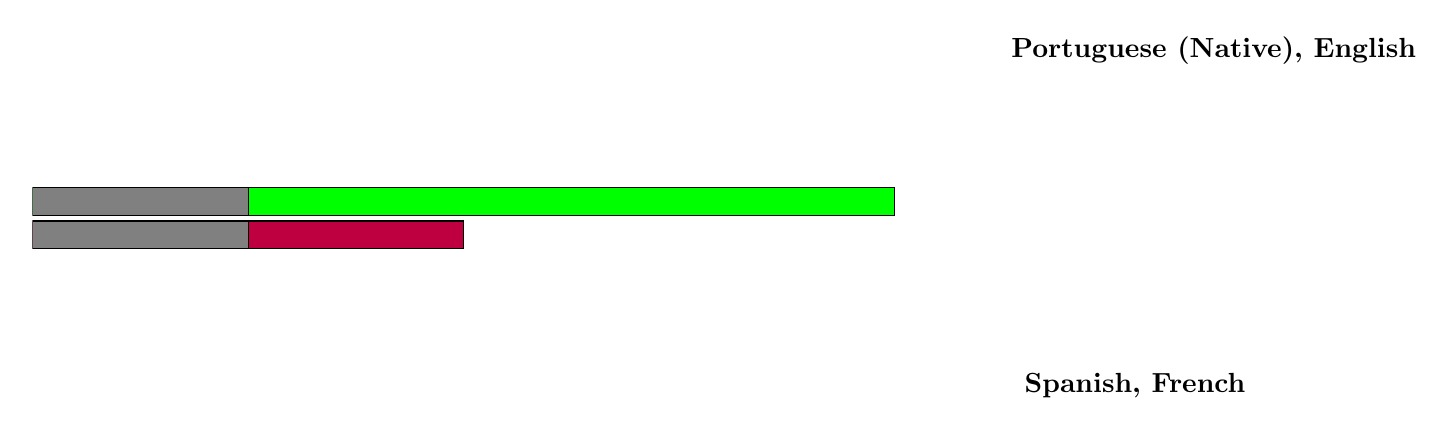
\begin{tikzpicture}
\begin{axis} [
	xbar, 
	height = 30mm, 
    width = 18cm,
	hide axis,
	xmin = 0,
	xmax = 36,
	%ymin = -0.1,
	%ymax = 0.1
]

\addplot [fill = purple] coordinates {
(6,0) (6+6,0) 
};
\addplot [fill = green] coordinates {
(6,0) (6+18,0) 
};



%Decription
\coordinate (A) at (1.4cm,3);
\coordinate (B) at (1cm,-3);

%CEFRL
\coordinate (C) at (3.8cm,3);
\coordinate (D) at (3.8cm,-3);

%Languages
\coordinate (E) at (15cm,3);
\coordinate (F) at (14cm,-3);

\end{axis}  

\begin{axis} [
	xbar, 
	height = 30mm, 
    width = 18cm,
	hide axis,
	xmin = 0,
	xmax = 36,
	%ymin = -0.1,
	%ymax = 0.1
]

\addplot [fill = gray] coordinates {
(6,0) 
};
\addplot [fill = gray] coordinates {
(6,0) 
};


\end{axis}  

\node at (A) {\textcolor{white}{\textbf{Proficient User}}};
\node at (B) {\textcolor{white}{\textbf{Basic User}}};

\node at (C) {\textcolor{white}{\textbf{CEFRL:C2}}};
\node at (D) {\textcolor{white}{\textbf{CEFRL:A2}}};

\node at (E) {\textbf{Portuguese (Native), English}};
\node at (F) {\textbf{Spanish, French}};

\end{tikzpicture}    

\vspace{0.5cm}